% !TEX encoding = UTF-8 Unicode
\section{Группы Ли}

\begin{defi}
Множество $G$ называется \textit{группой Ли}, если
\begin{enumerate}
\item $G$ — группа,
\item $G$ — гладкое многообразие,
\item отображения $(g,h)\mapsto gh$ и $g\mapsto g^{-1}$ — гладкие.
\end{enumerate}
\end{defi}

\begin{ass}
Пусть группа $G$ — множество решений гладких уравнений, тогда $G$ — группа Ли.
\end{ass}

\begin{examples} Следующие группы являются группами Ли
\begin{enumerate}
\item $\GL_n(\mathbb{R})=\{A\in \Mat_n(\mathbb{R})|\det(A)\neq 0\}$
\item $\SL_n(\mathbb{R})=\{A\in\Mat_n(\mathbb{R})|\det(A) = 1\}$
\item $\Ort_n(\mathbb{R})=\{A\in\Mat_n(\mathbb{R})|A^t=A^{-1}\}$
\item $\Aff(\mathbb{R})=\left\{\left(\begin{array}{cc}a & b \\0 & 1\end{array}\right)\left|\right.a\neq0;a,b\in\mathbb{R}\right\}$
\end{enumerate}
\end{examples}

\begin{defi}
Пусть $G$ — группа Ли, тогда подгруппа $H$ называется \textit{подгруппой Ли}, если $H$ — подмногообразие.
\end{defi}

\begin{defi}
Пусть $G$ — группа Ли, $G$ подгруппа Ли в $\GL_n(\mathbb{R})$. $X$ - косательный вектор к группе $G$ в точке $e$, если существует кривая $g(t)$ такая, что $\forall t\in\mathbb{R}:g(t)\in G, g(0)=e$ и $\frac{dg(t)}{dt}|_{t=0}=X$
\end{defi}

\begin{defi}
Множество всех касательных векторов в точке $e$ к группе $G$ называется касательным пространством и обозначается $T_e(G)$.
\end{defi}

\begin{ass}
Касательное пространство это подалгебра Ли в $\mathfrak{gl}_n(\mathbb{R})$.
\end{ass}

\begin{thm}
Пусть $\mathfrak{g}$ — алгебра Ли группы $G$, $H$ — подгруппа Ли в $G$, $\mathfrak{h}$ — алгебра Ли подгруппы $H$. Если $H$ — нормальная подгруппа в $G$, то $\mathfrak{h}$ — идеал в $\mathfrak{g}$.
\end{thm}

\begin{defi}
Путь из $p$ в $q$ — отображение $x:[0,1]\to X$ такое, что $x(0) = p,x(1)=q$.
\end{defi}

\begin{defi}
Многообразие $X$ называется связным, если $\forall p,q\in X$ существует непрерывный путь из $p$ в $q$.
\end{defi}

\begin{defi}
Многообразие $X$ называется односвязным, если любую петлю можно непрерывно стянуть в точку.
\end{defi}

\begin{ass}
Пусть $G$ — связная односвязная группа Ли, $\mathfrak{g}=\Lie(G)$, $\mathfrak{h}$ — подалгебра Ли в $\mathfrak{g}$, тогда в $G$ существует подгруппа Ли $H$ такая, что $\Lie(H)=\mathfrak{h}$.
\end{ass}

\begin{defi}
Пусть $G_1,G_2$ — группы Ли, $\phi:G_1\to G_2$. Отображение $\phi$ называется гомоморфизмом групп Ли, если
\begin{enumerate}
\item $\phi$ — гомоморфизм групп;
\item $\phi$ — гладкое отображение.
\end{enumerate}
Если $\phi$ — биекция, то $\phi$ называется изоморфизмом групп Ли.
\end{defi}

\begin{thm}
Если $\phi$ - гомоморфизм групп Ли, то $\Phi=d_e\phi:\mathfrak{g}_1\to\mathfrak{g}_2$ — гомоморфизм алгебр Ли.
\end{thm}

\begin{thm}
Пусть $G$ — подгруппа Ли в $\GL_n(\mathbb{R})$. Тогда $\mathbb{g}=\Lie(G)$ — подалгебра в $\mathfrak{gl}_n(\mathbb{R})$ и $exp:\mathbb{g}\to G$.
\end{thm}

\begin{ass}
Отображение $exp:\mathfrak{g}\to G$ — локальный диффеоморфизм окрестности нуля в $\mathfrak{g}$ на окрестности $e$ в $G$.
\end{ass}

\begin{thm}
Если $\phi$ — гомоморфизм групп Ли $G_1,G_2$, то $\Phi=d_e\phi$ — гомоморфизм алгебр Ли $\Lie(G_1),\Lie(G_2)$. Причем следующая диаграмма коммутативна
  $$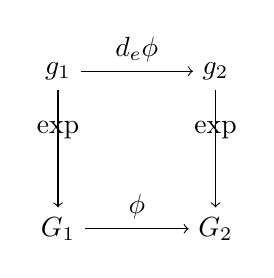
\begin{tikzpicture}
    \node (A) at (0,0) {$G_1$};
    \node (B) at (2,0) {$G_2$};
    \node (C) at (0,2) {$\mathfrak{g}_1$};
    \node (D) at (2,2) {$\mathfrak{g}_2$};
    \path [->] (A) edge [above] node {$\phi$} (B);
    \path [->] (C) edge [above] node {$d_e\phi$} (D);
    \path [->] (C) edge [above] node {$\exp$} (A);
    \path [->] (D) edge [above] node {$\exp$} (B);
  \end{tikzpicture}$$
  Т.е. $\forall x\in \mathfrak{g}_1:\exp\Phi(x)=\phi(\exp(x))$.
\end{thm}

